\section{Introduction}
\label{section:introduction}


% Reason

% Aim

% Structure


% Background and literature on the topic of floating islands, floating breakwaters, optimisation techniques and \acrfull{cfd} are summarized in Chapter \ref{ch: background and literature}. Out of this literature study the research objectives can be obtained, from which research questions are formulated in Chapter \ref{ch: research}. The methodology is presented in Chapter \ref{ch: PoA} and a project timeline with a rough day to day planning is shown in appendix \ref{appendix:project timeline}. 

\section{Background}
\label{sec:intro background}
Due to societal challenges such as the housing crisis in the western world and the impacts of climate change, there is an increasing shortage of safe living spaces. Therefore, there is an urgent societal need for alternative strategies that address the problem of increasing space shortage and, at the same time, are protected from natural forces such as flooding. An alternative solution would be the reclamation of land by sand nourishment; a process involving dredging sand from a source to feed the beach where land expansion is desired.  However, these processes become more expensive as the depth of the water increases. Therefore, the development of floating islands is more appealing, as it would be a more economical solution for many locations at sea where the water depth is high.  


% But to realise these floating cities, a few challenges need to be overcome. When a floating structure is placed at the surface of the sea, it will move due to the action of the waves. To minimize these motions, the dimensions of the structure need to be very large. But then the drift forces will be very high, so the mooring costs will become enormous. To reduce these drift forces, some of the wave energy needs to be attenuated with the help of a breakwater. How this breakwater can be designed best for this purpose is investigated in this master thesis. \\

\begin{figure}[h]
    \centering
    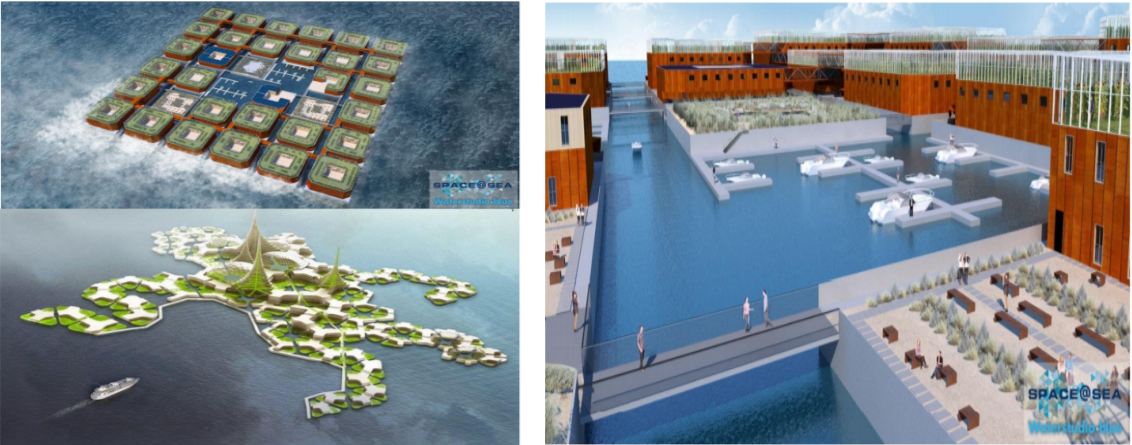
\includegraphics[width=\linewidth]{figures/Literature_Introduction/space@sea_renders.PNG}
    \caption{Living@Sea rendering for Space@Sea \citep{businessCase_S@S_D1.1}}
    \label{fig:my_label}
\end{figure}

The feasibility of floating islands is analysed in the 3-year project Space@Sea, whose main statement is; "Seventeen European partners aim to provide a sustainable and affordable workspace at sea by developing a standardised and cost-efficient modular island with low ecological impact" \citep{businessCase_S@S_D1.1}. This study was carried out for two different cases, where the first was located in the Mediterranean Sea, while the other was situated in the North Sea. The Mediterranean business case evaluated \acrshort{capex} (\acrlong{capex}: Major purchases that are designed to be used over the long term) are 49\% and \acrshort{opex} (\acrlong{opex}: Day-to-day expenses) are 99\% of its alternative: the fixed jacket. This difference in \acrshort{capex} is due to the deep water characteristics of the Mediterranean, where a soft mooring system (of a floating island) would be much cheaper instead of jackets fixed to the bottom of the sea. The alternative in the North Sea was land reclamation, which is possible here due to the low water depth. Therefore, the costs of a floating island were compared to the costs of constructing an island by land reclamation in the North Sea business case. The \acrshort{capex} of a floating island would be 183\% and its \acrshort{opex} 138\% of the \acrshort{capex} and \acrshort{opex} of its competitor, due to the high costs of the current design of the mooring system. Due to the geographical position of the floating island, the northern swell in the North Sea can deliver waves with a wave height of up to nine metres, resulting in high \acrshort{capex} (owing to high mooring costs) and \acrshort{opex} (due to maintenance of the modules and connectors). The wave height is determined by the wind, the distance from the upwind coastline (\textit{fetch}) and the time since the wind started blowing \citep{Holthuijsen2007}. The location studied in the North Sea is at 51$\deg$ N, 3$\deg$ S (see the green mark in Figure \ref{fig:locationNS}), so when the wind comes from the north-northwest, the fetch reaches all the way up to the Arctic Sea, resulting in waves coming from this direction that can get immense under certain conditions.

\begin{figure}[H]
    \centering
    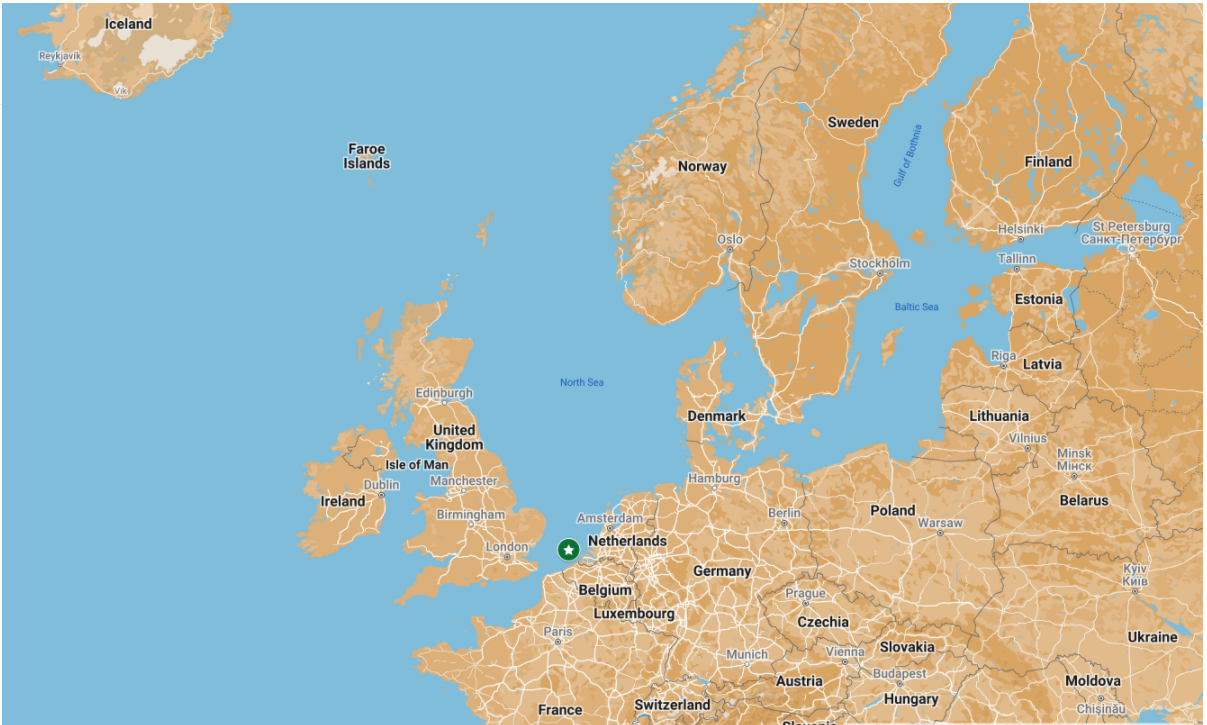
\includegraphics[width=1\linewidth]{figures/Literature_Introduction/location_NS.PNG}
    \caption{Location floating island North sea}
    \label{fig:locationNS}
\end{figure}

Breakwaters, connected to the wave-ward side of floating islands, can provide shelter by attenuating waves through dissipation and reflection. Therefore, they contribute to increasing the number of possible locations where such a floating island could function in the future. Many studies have been conducted on the topic of breakwaters (which are addressed in Chapter \ref{ch:literaturereview}), yet never with a connection to a large structure such as a floating island in this case. \\
\\
Furthermore, there is a knowledge gap in using design optimisation with ComFLOW in combination with the study of breakwaters, and the validation of ComFLOW's results regarding the mean wave drift force on box-type breakwaters interacting with regular waves has not been executed before. 


\section{Problem statement}
Wave drift forces are a consequence of wave loads. These forces cause the floating structure, when freely floating in waves, to drift in the direction of propagation of the waves due to the second-order wave forces \citep{journee2000offshore}. The mooring system is there to provide the counter force to keep the structure in its place. When the mean wave drift force on the structure increases, its required mooring system becomes more expensive. The magnitude of these second-order wave drift forces scales quadratically to the height of the waves. Therefore, the mooring costs are highly dependent on the height of the incoming waves.\\
\\
% Furthermore, the individual modules of a floating island will move with respect to each other under the action of waves. The fenders (connectors between the different modules) are designed to keep the modules together as one floating structure and will therefore need to withstand loads. The higher these loads are, the more robust and expensive the fenders need to be. So, also the fender costs are dependent on the height of the waves interacting with the structure.\\
% \\



Therefore, to make floating islands an applicable option to provide living/working spaces at sea, the energy of the waves must be dissipated and reflected with the help of a breakwater with an optimised geometry. Research questions are being developed from which thorough research is needed to answer them. This is then required to achieve this objective.

% Because both the construction and maintenance costs of the floating island depend strongly on the height of the waves interacting with the structure, it is economically beneficial to come up with way to attenuate the incoming waves. A breakwater can serve this purpose by dissipating and reflecting wave energy. 


\section{Research questions}
\label{sec: research questions}
The main objective is to attenuate the waves that interact with the structure and thus lower the drift forces and the hydroelastic response of the floating island. Lowering the drift forces will lead to a reduction in the mooring costs, and lowering the motions of the individual modules will lead to an increase in the workability of the island. Due to the infinite number of possible geometries of the floating breakwater and the various external conditions in which it must operate, the optimisation's \textit{design space} is large. Therefore, optimisation will be used to come up with a final design. This main objective is formulated as a question and therefore is the main research question for this thesis: 

\begin{enumerate}
    \item How can the construction costs of a floating island be reduced by connecting a structure to its wave-ward side with an optimised geometry?
\end{enumerate}


The sub-research questions are formulated as follows:
\begin{enumerate}[resume]
    \item What is the quality of the results of ComFLOW with the best possible settings?
    \item How do wave attenuation and reduction of drift forces relate to the geometry of the breakwater?
    \item How are the drift forces and the geometry of the breakwater quantified in mooring and construction costs, respectively?
\end{enumerate}





%\section{Research approach}

% -right grid 
% -validation ComFLOW, reflection and dissipation


% -optimisation between ComFLOW and optimisation method, which is considering the which evaluations to compute

% -design of experiments



\section{Report structure}
This report is structured as follows:


\begin{itemize}
    \item In Chapter \ref{ch:literaturereview} a review of the literature can be found on the studies of floating islands, floating breakwaters, wave forces on marine structures, optimisation techniques and \acrfull{cfd}, with ComFLOW in particular. 
    \item Chapter \ref{ch: methodolgy} describes extensively the methodology of this thesis, with the setup of the optimisation, the post-processing of ComFLOW results and the cost function which calculates the cost reduction each breakwater delivers.
    \item In Chapter \ref{ch: validation comflow} the validation of ComFLOW is discussed. This resulted in certain settings and a grid. Also, a comparison is made with the results of ComFLOW with linear wave theory and an experiment in which waves plunged over a breaker bar. 
    \item An hydrodynamic design optimisation is given in Chapter \ref{ch: captive design optimisation}, where the link is made between the geometry of the breakwater and its hydrodynamic performance. 
    \item An economic design optimisation is given in Chapter \ref{ch: economical design optimisation } to obtain the optimal geometry of the breakwater regarding the reduction in capital expenditure.
    \item Finally, the conclusions and recommendations are presented in Chapter \ref{ch: conclusions recommendations}.
\end{itemize}

